\documentclass[a4paper,11pt]{article}


\usepackage{geometry} % for making easy changes to page layout
\geometry{body={15cm,24cm}} % change height and width of main text
\usepackage{yhmath}

\usepackage{parskip} % for blank lines between paragraphs 
\usepackage{bbm}
\usepackage{minted}

\usepackage{amsmath,amssymb} % for serious mathematics, such as \begin{align*} etc

\usepackage{graphicx} % for \includegraphics[width = 1\textwidth]{} etc
\usepackage{booktabs}

\title{GLM Practical}
\author{P806}
\date{7 December 2022}

\begin{document}

\newcommand{\E}{\mathrm{E}}

\newcommand{\Var}{\mathrm{Var}}

\newcommand{\Cov}{\mathrm{Cov}}

\maketitle

\section{Introduction}
The presented dataset consists of 5190 responses to a survey about doctor visits. For each response, the number of doctor visits in the two weeks before the survey is the response variable, and information about the age, gender, income, insurance, and chronic diseases is recorded about the respondents. Hence the design of the dataset is
\begin{align*}
\centering
\mathbf{x}  & \longmapsto y \\
\mathbf{x} &= (\text{Age, Gender, Income, Type of Insurance, Chronic Condition}) \\
 &= (x^{(a)}, x^{(g)}, x^{(i)}, x^{(t)}, x^{(c)}) \\
y &= \text{Number of Doctor Visits in preceding two weeks} \in \mathbb{N}
\end{align*}
$x^{(a)}$ and $x^{(i)}$, the age and the income of survey respondents, are real numbers, while $x^{(t)}$, $x^{(g)}$, and $x^{(c)}$ are categorical variables.

Note that in the raw dataset, there is no column on insurance type, but the insurance type is constructed from the columns \texttt{private, freepoor, freerepat}. Those columns are binary indicator variables for the three insurance types, and they are never all \texttt{1} for any sample. So, we create a variable \texttt{insurance} that is a categorical variable and has four different possible values: \texttt{private, freepoor, freerepat}, and \texttt{normal}. $\texttt{insurance} = \texttt{normal}$  if \texttt{private, freepoor, freerepat} are all $0$ in the original dataset.

Similarly, there is not actually a \texttt{gender} variable in the dataset, but only a binary indicator if the respondent was female or not. For simplicity, we convert that indicator into a categorical variable that has the values \texttt{male} and \texttt{female}.
\begin{figure}[h]
	\centering
	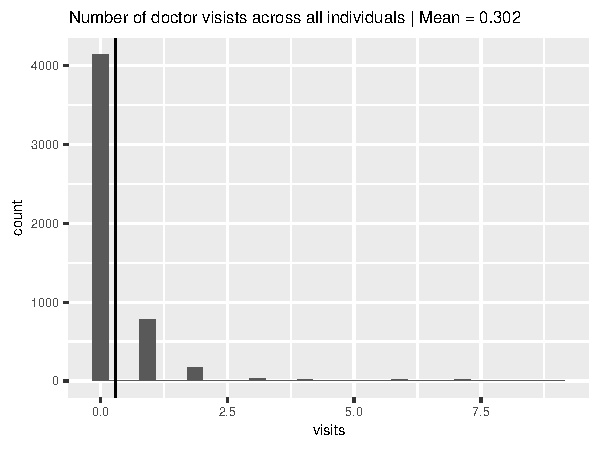
\includegraphics{../plots/histogram_of_visits.pdf}
	\caption{Histogram of entire dataset}
	\label{fig:hist_all}
\end{figure}

\section{Data Exploration}
First, looking at figure \ref{fig:hist_all}, we see that a large majority of the survey answers are $0$. The mean response is $0.302$. Considering that we are counting occurrences of events and the large zero-count, a Poisson model lends itself as a possible model to fit to the data. 

Figure \ref{fig:hist_insurances} gives a first glimpse into the relationship of $\mathbf{x}$ and $y$. We see the same plot as in figure \ref{fig:hist_all}, but for the dataset split by the type of insurance the survey respondents had. We see that the type of insurance has some influence of the mean number of visits to the doctor. In particular, people with free government insurance due to old age, disability, or veteran status, i.e., $x^{(t)} = \texttt{freerepat}$ have a much higher mean number ($0.4665$) of doctor visits than people with other type of insurance. 

\begin{figure}[h]
	\centering
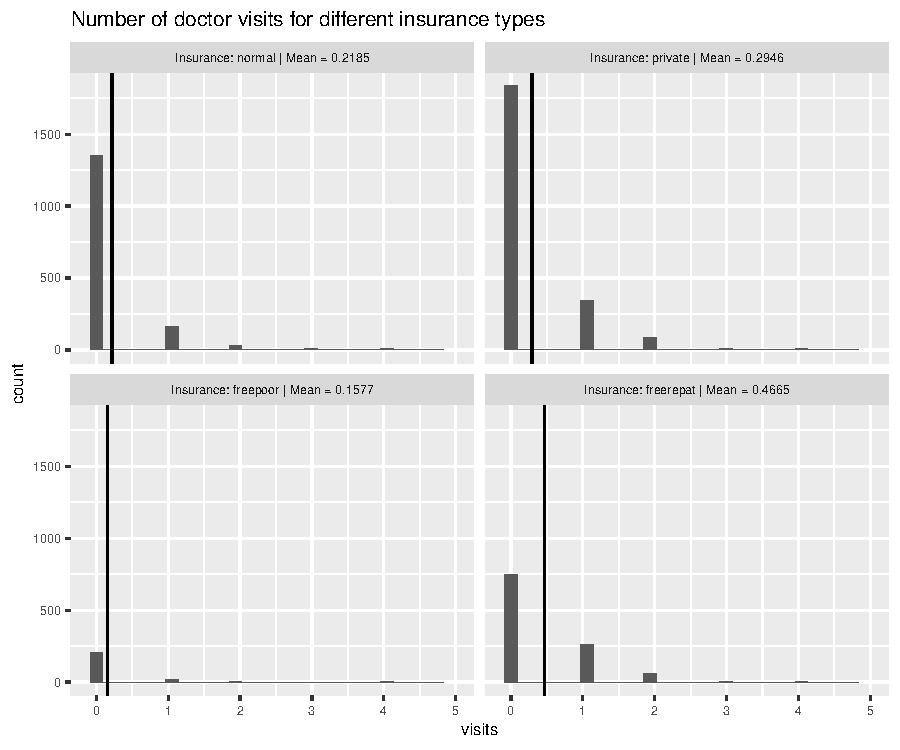
\includegraphics{../plots/histograms_of_insurances.pdf}
		\caption{Histogram of data split by type of insurance}
			\label{fig:hist_insurances}
\end{figure}

This is supported by table \ref{tab:stats_fine}. We see that the mean number of doctor visits of respondents with the \texttt{freerepat} insurance is the highest. This might be because the insurance has an influence on the number of doctor visits, or because the respondents with that insurance had a higher age on average. Additionally, the number of doctor visits from those patients has the highest variance. In general, we see that the variance of doctor visits increases with increasing mean.

\input{../report/descriptive_stats_fine.txt}

Table \ref{tab:stats_coarse} shows the doctor visits split by gender. We see that females have a higher mean number of visits and a higher variance of visits. But it also comes apparent that this might actually be the case because the sample includes women of a higher age, on average.

\input{../report/descriptive_stats_coarse.txt}

In order to understand if the age has an influence on the number of doctor visits, we refer to figure \ref{fig:scatter_income_and_age}. There, we see nicely how the mean number of doctor visits \emph{decreases} with increasing income and \emph{increases} with increasing age. We might thus postulate the hypotheses that the mean number of doctor visits depends on age and income. We shall further investigate this hypothesis in the next section.

\begin{figure}[h]
	\centering
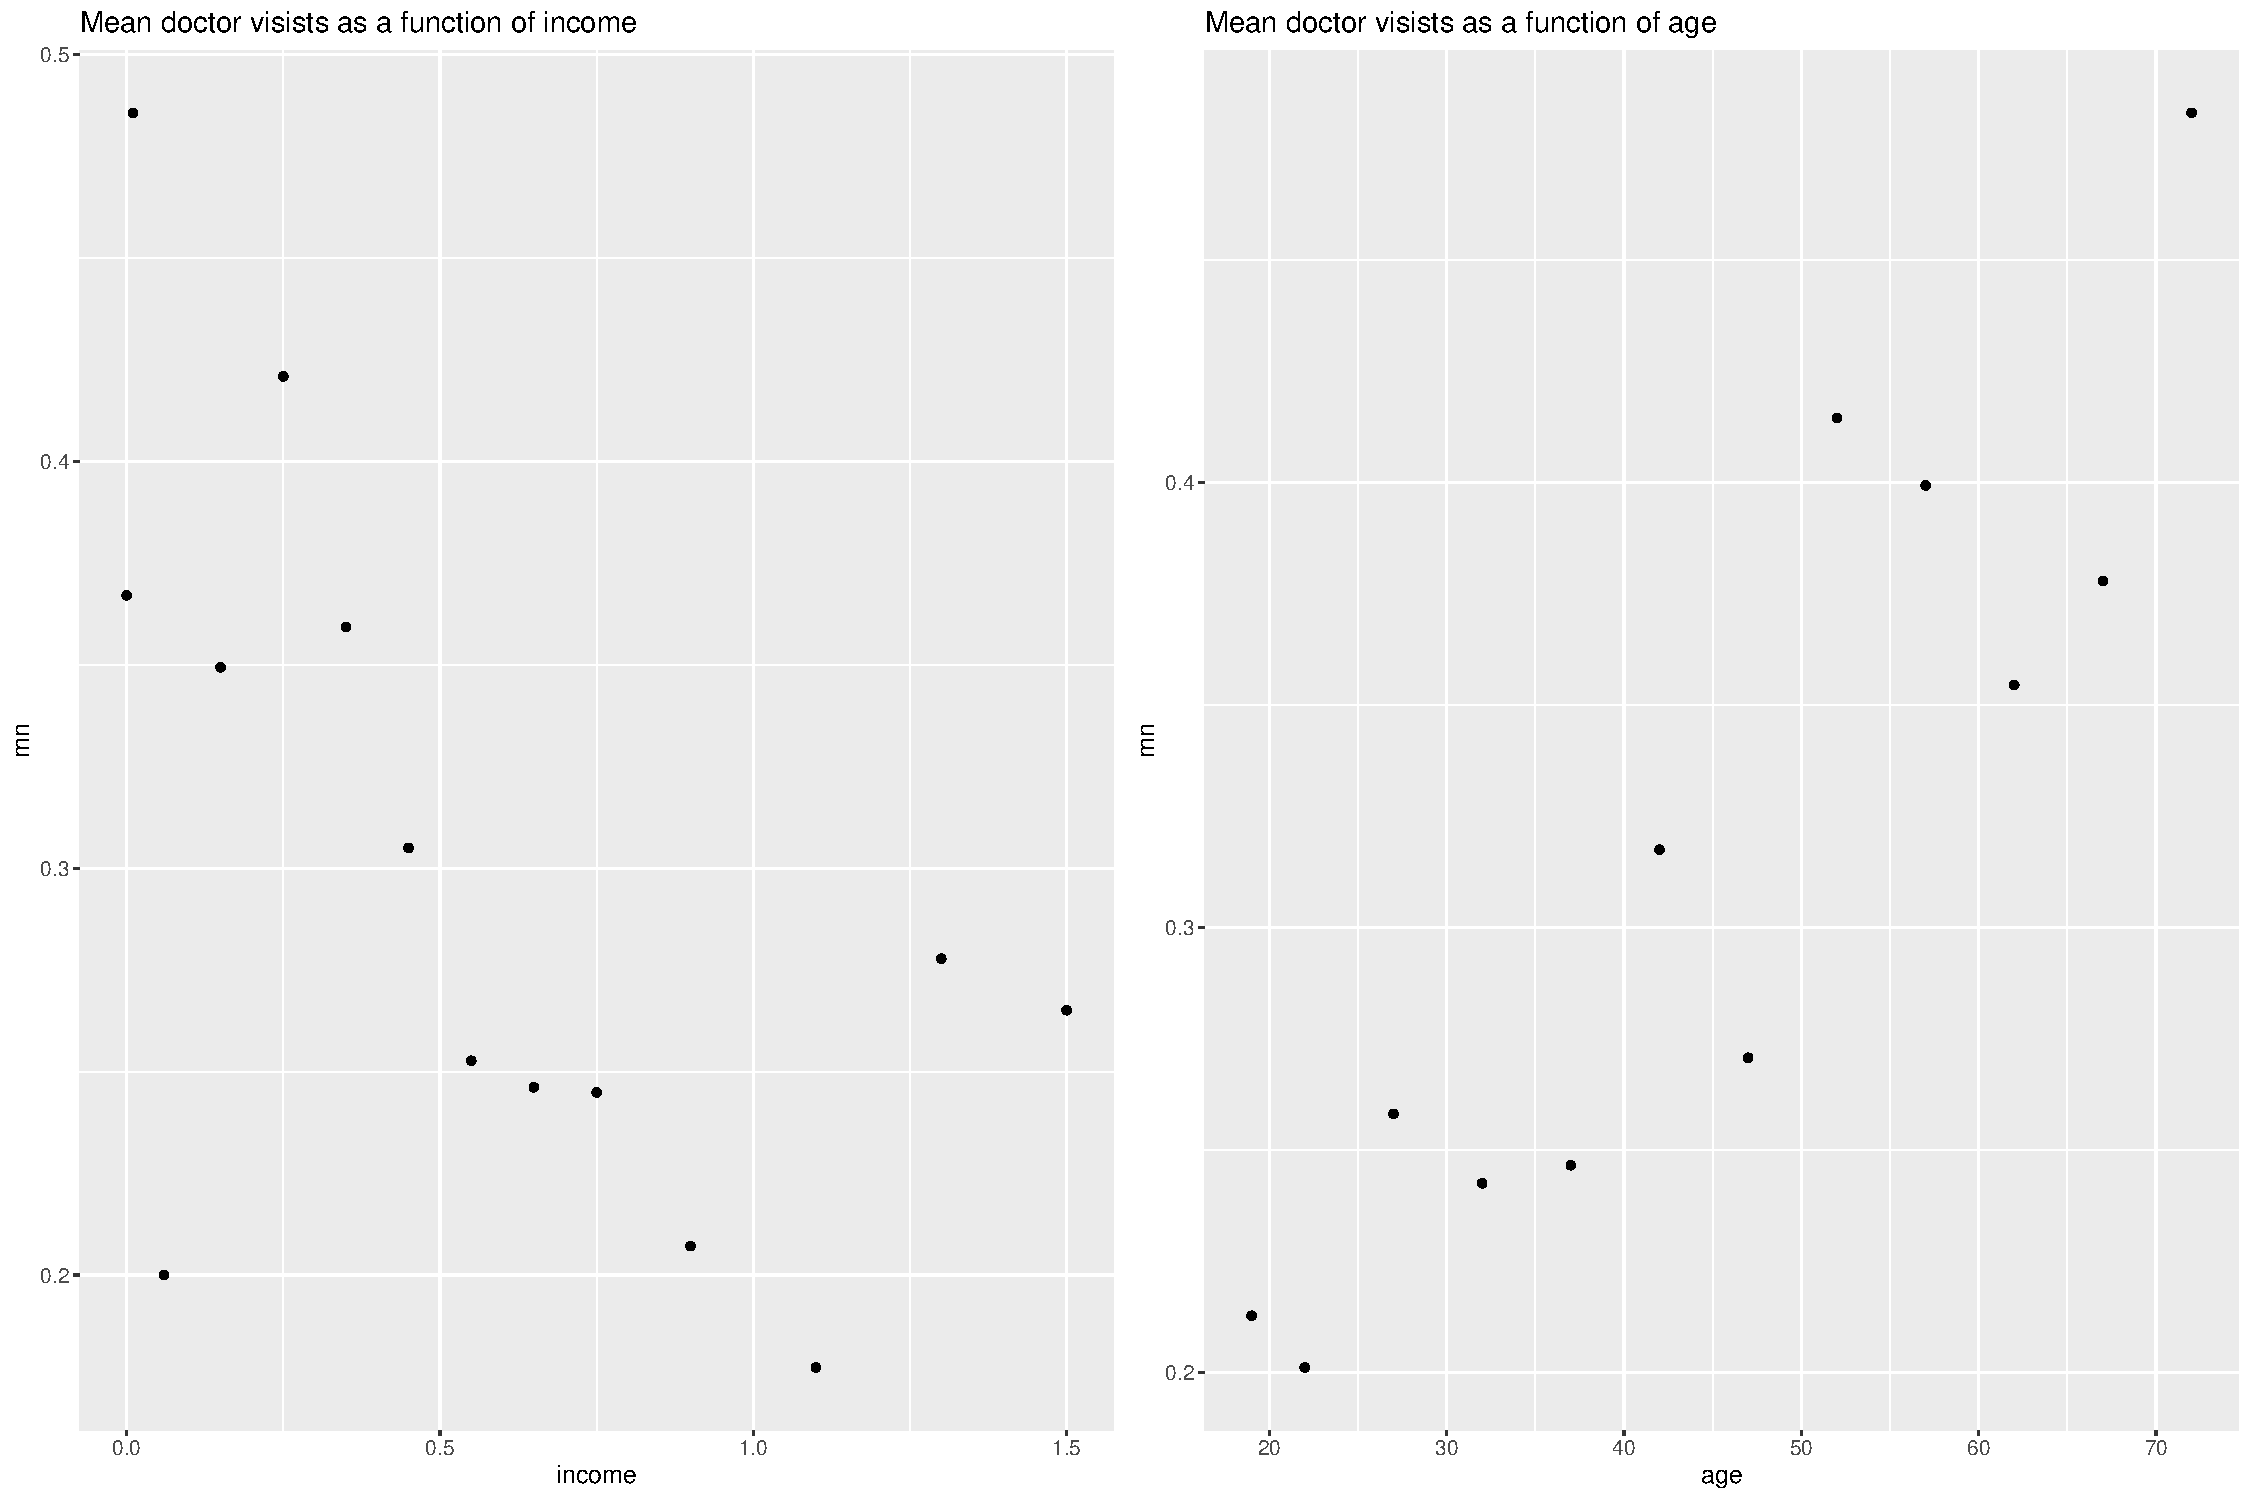
\includegraphics{../plots/mean_vs_income_and_age.pdf}
	\caption{Mean doctor visits as a function of income (left) and age (right)}
		\label{fig:scatter_income_and_age}
\end{figure}

\begin{figure}[h]
	\centering
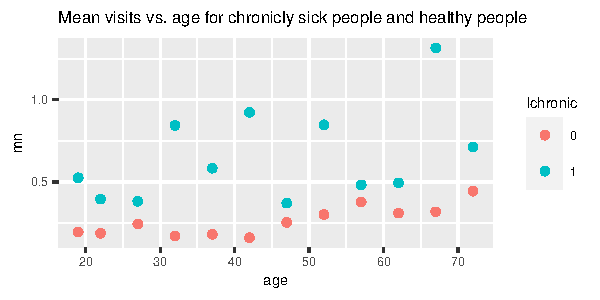
\includegraphics{../plots/mean_vs_age_and_chronic.pdf}

\caption{Mean doctor visits as a function of age for responses of chronically ill and healthy people}
\label{fig:scatter_age_and_chronic}
\end{figure}

For the impact of chronic diseases, we refer to figure \ref{fig:scatter_age_and_chronic}.  That plot shows the mean number of doctor visits as a function of respondent age, split by the value of $x^{(c)}$. From that plot, we may hypothesize that having a chronic disease increases the number of doctor visits. 

\subsection{Domain check on continuous variables}

We should make sure that all variables are in a domain that makes sense in the real world, i.e., we should impose maximum and minimum values on \texttt{age}, \texttt{income}, and \texttt{visits}. Table \ref{tab:min-max} shows the extrema for all those variables in the dataset. We see that there are no samples out of the range of reasonable values, hence we can include all samples in the analysis.

\begin{table}[h]
\centering
\begin{tabular}{l|r|r}
\hline
Variable & Min & Max\\
\hline
Age & 19 & 72 \\
Income & 0 & 1.5 \\
Visits & 0 & 9 \\
\hline
\end{tabular}
\caption{Minimum and maximum values for real variables}
\label{tab:min-max}

\end{table}


\section{Modelling of the Relationship}
In the assignment, we were asked to develop a Poisson model with canonical link function. Thus, the relationship of $y_i$ and $\mathbf{x_i}$ is:
\begin{align}
& y_i \sim \text{Poisson}(\lambda_i) \\
&\lambda_i = \exp{\eta_i} = \exp(\mathbf{x_i}^T\beta)
    \label{eq:model}
\end{align}
Since for the Poisson model we have $\mu = \lambda$, we see that the canonical link function in this case is $\eta = g(\mu) = \log(\mu)$.

The assignment further aksed us to only consider the interaction term of the gender feature, $x^{(g)}$ with the other features of $\mathbf{x}$. The model with all those allowed interaction terms can be created in \texttt{R} with the following command:

\begin{verbatim}
glm(visits ~ . + gender*., data = df, family = poisson(link = log))
\end{verbatim}

After fitting this simple model, we analyze the z scores for the different coefficients of $\hat{\beta}$. The z values for many coefficients suggest that it is quite likely that they are zero. Hence, we use a backwards AIC search to set certain estimates $\hat{\beta}_j$ to zero.  This is conducted with the \texttt{stepAIC} method from the \texttt{MASS} package for \texttt{R}.

The backwards feature elimination finds that the interaction terms of the gender with the income, the chronic disease indicator, and the categorical variable for the type of insurance should be removed.

\begin{table}[h]
    \centering
    \begin{tabular}{l|l|r|r|r}
    \hline
 \# &Model & AIC & Deviance & $R^2$\\
    \hline
1&    Baseline Model with all features ($p=14$) &  7631.499 & 5271.931 & 0.0644\\
2&    After backwards feature elimination ($p=9$) & 7624.555 & 5274.988  & 0.0639\\
        \hline
        
    \end{tabular}
    \caption{Table of model diagnostics for the full model and the reduced model}
    \label{tab:backwards_elimination}
\end{table}
In table \ref{tab:backwards_elimination}, we show the AIC, deviance and the generalized $R^2$ metric as defined by \cite{cameron}. The table nicely shows how the removal of the 5 interaction coefficients in $\hat{\beta}$ reduces the AIC while slightly increasing the deviance and $R^2$ metric of the model, as expected. Note that we still chose the model with higher deviance and lower $R^2$ metric, because our model selection criterion is the AIC to get an explainable model with manageable $p$.

Given that we have the hypothesis that five parameters of the initial $\hat{\beta}$ may be $0$, so we can construct a hypothesis test to confirm or reject it. For this, we refer to section 4.4.3 of the lecture notes and use that, for $r<p$ we have:
\begin{equation}
D^{(r)}(y) - D^{(p)}(y) \sim \chi^2_{(p-r)}
\end{equation}
Now, the difference in the deviances turns out to be $3.06$, and the difference in number of parameters is $5$. Also, we have that $\mathbb{P}( \chi^2_{5} > 3.06) = 0.691$. Hence we do not have to reject the hypothesis and we can move on with the model with the smaller number of parameters.

\section{Assessing model fit}
The most straightforward way to assess the model fit is to look at the scaled deviance of the model, $D(y)$. When the model is well fit, we expect $D(Y) \sim \chi^2_{(n-p)}$. With $D(y) = 5275$, $n = 5190$, and $p=9$, we have $\mathbb{P}( \chi^2_{5181} > 5275) = 0.178$. Although this is quite small, we do not have to reject this model at the $5\%$ acceptance limit. Also, note that for this data we do not expect the $\chi^2$ approximation for $D(y)$ to be perfect, since we have small counts in the Poisson.

One could also look at the standardized deviance and standardized Pearson residuals. As discussed in the lectures, those residuals are not expected to be standard normals, but they should have unit variance. We thus compute the standardized deviance residuals with the \texttt{R} command \texttt{rstandard} and find that the variance of those residuals is, in fact, $0.92$. Hence, the variance of the residuals is in the expected range, although it is a little smaller than expected.

Table \ref{tab:estimates} lists the p-values for the model coefficients. We see that the three parameters for the insurance are quite likely to be zero. Nevertheless we choose to include those coefficients, since the number of available variables is quite small. It should be noted though, that the influence of the insurance on a person's doctor visits is small, if not negligible!
\input{outlier-data.txt}

When computing the Cook's Distance for every sample and comparing it to $8/(n-2p)$, we count 170 outliers. We show the data for the 5 samples with the highest Cook's Distance in table \ref{tab:outlier-data}. There is nothing that is unreasonable about those samples, so we decide to keep all outliers in the dataset and move on with the model fitted on all samples.

\section{Model Interpretation}

We list all parameter estimates, their confidence intervals and means ratios in table \ref{tab:estimates}. Going back to equation \ref{eq:model}, the linear predictor has the form
\begin{align}
\eta_i &= \beta_0  +  \beta_2 x^{(i)} + \beta_3 \mathbbm{1}\{x^{(g)} = \text{"female"}\}     +\beta_4\mathbbm{1}\{x^{(c)} = 1\}   + 
 \beta_5\mathbbm{1}\{x^{(t)} = \text{"private"}\}    \nonumber\\
 &+  \beta_6\mathbbm{1}\{x^{(t)} = \text{"freepoor"}\}  + \beta_7 \mathbbm{1}\{x^{(t)} = \text{"freerepat"}\}  \\
&+   x^{(a)}(\beta_8 \mathbbm{1}\{x^{(g)} = \text{"female"} \} + \beta_1) \nonumber
\end{align}

Coming back to the interpretation of confidence intervals, we can say that, e.g. for $\beta_1$ (the coefficient for the age of male respondents), upon repeating the same sampling from the population, the true parameter $\beta_1$ will be in 95\% of the confidence intervals.

Now, we shall look at the means ratios. For example, the means ratio for the chronic disease state is $2.034$. This means that the expected number of doctor visits doubles if a respondent has the chronic disease and all other features are the same. Moreover, an increase in income of ten thousand dollars will reduce the expected number of doctor visits by about 25\%.

\input{../report/estimates.txt}

We also see that the means ratio for the age feature is $1.016$ for a male respondent. So, for an increase of 10 years in a male respondent's age, the expected number of doctor visits will be multiplied by $1.016^{10} = 1.17$, i.e., it will increase by about 17\%. 

\begin{table}[h]
\centering
\begin{tabular}{l|l|r|r|l|r|}
\hline
Feature & Coefficient & $\hat{\beta}$ & CI $\hat{\beta}_i$ & MR & CI MR\\
\hline
         Age (for women)& $\beta_a $ & 0.0048&[0.0012, 0.0084]& 1.0048 &[1.0029, 1.0066] \\
\hline
 \end{tabular}
 \caption{\label{tab:femal_age}Parameter estimate and means ratios(MR)
             with its 0.95 confidence intervals}
\end{table}

The influence of the age is slightly different for females compared to males. Let's define $\beta_a = \beta_8 + \beta_1$, the coefficient for the age variable, $x^{(a)}$, of females. Then, the approximate variance of that estimate is:
\begin{equation}
\widehat{\Var}(\hat{\beta}_a) = \widehat{\Var}(\hat{\beta}_8) + \widehat{\Var}(\hat{\beta}_1) + 2 \widehat{\Cov}(\hat{\beta}_8, \hat{\beta}_1)
\end{equation}
Further, we can get the means ratio for an age increase of a female respondent:
\begin{equation}
M^a = \exp(\beta_a) = \exp(\beta_8 + \beta_1)
\end{equation}
With all of this, we find the numeric values shown in table \ref{tab:femal_age}.
So, we see that the effect of age is very small for women. For a ten year increase in the age, women are expected to go $1.0048^{10} = 1.05$ times more often to the doctor. Hence, the increase for 10 years is 5\% for women compared to 17\% for men. 

We now want to interpret the model as to how the doctor visits are influenced by the gender, when all other variables are fixed. Let $\mu_M$ and $\mu_F$ be the expected number of doctor visits for male and female respondents that have every feature of $\mathbf{x}$ the same except for the gender. Then, we have that 

\begin{equation}
\frac{\mu_F}{\mu_M} = \exp(\beta_3 + x^{(a)}\beta_8) = 2.045\cdot (0.989)^{x^{(a)}}
\end{equation}

where  $x^{(a)}$ is the age of the man and the woman. Taking, for example, a woman of age $35$, we get that she has an expected number of doctor visits that is $1.37$ times the expected number of doctor visits of a similar male. For a female of age $65$, that number changes to $0.97$, i.e., 65 year old women are expected to go to the doctor less than comparable males.

We also have that 

\begin{equation}
\widehat{\Var}(\hat{\beta}_3 + x^{(a)}\cdot\hat{\beta}_8) = \widehat{\Var}(\hat{\beta}_3) +  (x^{(a)})^2 \widehat{\Var}(\hat{\beta}_8) + 2 \cdot x^{(a)}\cdot \widehat{\Cov}(\hat{\beta}_8, \hat{\beta}_3)
\end{equation}

So, the standard error of the impact of the gender scales with the age of the respondents. For a female of age 35, the 95\% confidence interval of the gender's influence is $[1.212, 1.54]$, while for the female of age 65, it is $[0.836 , 1.12 ]$. The standard errors are $0.0612$ and $0.0746$, respectively.

\section{Estimating the dispersion parameter}
In the lecture notes, we saw that 
\begin{equation}
\widehat{\phi} = \frac{1}{n-p} \sum_{i=1}^n \frac{(y_i- \hat{\mu}_i)^2}{V(\hat{\mu}_i)} = \frac{1}{n-p} \sum_{i=1}^n r_{P;i}^2
\end{equation}
Where $r_{P;i}$ is the (non-standardized) Pearson residual for sample $i$. Computing this in \texttt{R} yields an estimate of $\hat{\phi} = 1.992$. However, the real value for $\phi$ is $1$ in the Poisson model. Hence we should question whether the Poisson model, or the canonical link function, was actually a good choice in the first place. The fact that $\phi > 1$ indicates that the estimate for the variances of the $\hat{\beta}_i$ are actually too small and the p-values are too optimistic.

\section{Summary}
We have seen that the number of doctor visits in a two-week period can be described by a Poisson model, although other models could yield a better fit. The expected number of doctor visits largely depends on the age  and income of survey respondents, as well as any chronic diseases they have. The gender is important, because it changes how the age influences the number of doctor visits: Females have higher number of doctor visits at a young age, although men will go to the doctor a similar, if not higher, amount at higher age.

\bibliographystyle{plain}
\bibliography{refs}

\newpage

\section{Appendix}
\subsection{Data Loading and Manipulation Script}
\begin{minted}[linenos]{R}
get_eda_data <- function() {
  df <- read.csv("data/docvis.csv")
  df <- df %>%
    mutate(female = replace(female, female == 1, "female")) %>%
    mutate(female = replace(female, female == 0, "male"))
  df$female <- factor(df$female, levels = c("male", "female"))
  names(df)[names(df) == 'female'] <- 'gender'
  df$lchronic <- as.factor(df$lchronic)
  df[, "insurance"] <- "normal"
  df <- within(df, {
    insurance[df$private == 1] <- "private"
    insurance[df$freepoor == 1] <- "freepoor"
    insurance[df$freerepat == 1] <- "freerepat"
  } )

  df$insurance <- factor(df[, "insurance"],
                         levels = c("normal", "private", "freepoor", "freerepat"))

  subset(df, select = -c(private, freepoor, freerepat))
}
\end{minted}
\subsection{EDA Script}
\begin{minted}[linenos]{R}
setwd("/Users/konrad/code/school/MT/glm-practical")
source("helpers.R")
library(ggplot2)
library(dplyr)
library(tidyr)
library(gridExtra)
library(knitr)
library(kableExtra)

options(digits = 3)

# Define some constants - widths and heights in inches
FONT_SIZE <- 7
DOUBLE_FONT_SIZE <- 8
WIDTH <- 4
DOUBLE_WIDTH <- 6
DOUBLE_HEIGHT <- 3
HEIGHT <- 2

# use method from helper package
df <- get_eda_data()

## SECTION 1: PLOTTING ##

# Make a histogram of all the reponses together
ggplot(df) +
  geom_histogram(aes(visits)) +
  geom_vline(xintercept = mean(df$visits)) +
  ggtitle(paste("Number of doctor visists across all individuals | Mean =",
                round(mean(df$visits), 3))) +
  theme(text = element_text(size = FONT_SIZE)) +
  xlab("Visits") +
  ylab("Count of Respondents") +
  xlim(-0.25, 8)
ggsave("plots/histogram_of_visits.pdf",
       width = WIDTH, height = HEIGHT)

# Make plots by income and age
# First: group data by income only
df.grouped <- df %>%
  group_by(income) %>%
  summarise(n(), max(visits), min(visits), mn = mean(visits))
p1 <- ggplot(df.grouped, aes(income, mn)) + geom_point()
p1 <- p1 + ggtitle("Mean visists as a function of income")
p1 <- p1 +
  theme(text = element_text(size = DOUBLE_FONT_SIZE)) +
  xlab("Income") +
  ylab("Mean Visits")

# Second: group data by age only
df.grouped <- df %>%
  group_by(age) %>%
  summarise(n(), max(visits), min(visits), mn = mean(visits))
p2 <- ggplot(df.grouped, aes(age, mn)) + geom_point()
p2 <- p2 + ggtitle("Mean doctor visists as a function of age")
p2 <- p2 +
  theme(text = element_text(size = DOUBLE_FONT_SIZE)) +
  xlab("Age") +
  ylab("Mean Visits")

ggsave("plots/mean_vs_income_and_age.pdf",
       arrangeGrob(p1, p2, nrow = 1, ncol = 2),
       width = DOUBLE_WIDTH, height = HEIGHT)

# Make a histogram how the insurance influences how often people go
# Compute mean number of visits for different insurance types
ins.means <- df %>%
  group_by(insurance) %>%
  summarise(mn = mean(visits))
labels <- list()
for (value in ins.means$insurance) {
  m <- ins.means[ins.means$insurance == value, "mn"]
  label <- paste("Insurance:", value, "| Mean =", round(m, 4))
  labels[value] <- label
}
# now make a histogram divided by insurance type
p <- ggplot(df, aes(visits)) +
  geom_histogram() +
  facet_wrap(~insurance, labeller = as_labeller(unlist(labels))) +
  geom_vline(aes(xintercept = mn), ins.means) +
  xlim(-0.1, 5) +
  ggtitle("Number of doctor visits for different insurance types") +
  theme(text = element_text(size = DOUBLE_FONT_SIZE)) +
  xlab("Visits") +
  ylab("Count of respondents")

ggsave("plots/histograms_of_insurances.pdf",
       width = DOUBLE_WIDTH, height = DOUBLE_HEIGHT)


# Make a histogram how the gender influences how often people go
means <- df %>%
  group_by(gender) %>%
  summarise(mn = mean(visits))
labels <- list()
for (value in means$gender) {
  mean <- means[means$gender == value, "mn"]
  label <- paste("Gender:", value, "| Mean =", round(mean, 4))
  labels[as.character(value)] <- label
}
p <- ggplot(df, aes(visits)) +
  geom_histogram() +
  facet_wrap(~gender, labeller = as_labeller(unlist(labels))) +
  geom_vline(aes(xintercept = mn), means) +
  xlim(-0.1, 5) +
  theme(text = element_text(size = DOUBLE_FONT_SIZE)) +
  xlab("Visits") +
  ylab("Count of Respondents")
ggtitle("Number of doctor visits for different genders")
ggsave("plots/histograms_of_genders.pdf",
       width = DOUBLE_WIDTH, height = HEIGHT)

# Make a plot that shows the chronic diseases impact
df.grouped <- df %>%
  group_by(age, lchronic) %>%
  summarise(n(), max(visits), min(visits), mn = mean(visits))
ggplot(df.grouped, aes(age, mn, color = lchronic)) +
  geom_point() +
  theme(text = element_text(size = FONT_SIZE)) +
  ggtitle("Mean visits vs. age for chronicly sick
    people and healthy people") +
  xlab("Age") +
  ylab("Mean Visits") +
  labs(colour = "Chronic\nDisease")
ggsave("plots/mean_vs_age_and_chronic.pdf",
       width = WIDTH, height = HEIGHT)

## SECTION 2: CREATING SOME SUMMARY STATISTICS ##
df.grouped <- df %>%
  group_by(insurance) %>%
  summarise(n = n(),
            "mean age" = mean(age),
            "mean visits" = mean(visits),
            "variance of visits" = var(visits)
  )
# Output table to Latex
latex.table <- kable(df.grouped, "latex",
                     caption = "Descriptive statistics of
                     the dataset by insurance",
                     label = "stats_fine", position = "h")

fileConn <- file("report/descriptive_stats_fine.txt")
writeLines(latex.table, fileConn)
close(fileConn)

df.grouped <- df %>%
  group_by(gender) %>%
  summarise(n = n(),
            "mean age" = mean(age),
            "mean visits" = mean(visits),
            "variance of visits" = var(visits)
  )
latex.table <- kable(df.grouped, "latex",
                     caption = "Descriptive statistics of the
                     dataset by gender",
                     label = "stats_coarse", position = "h")

fileConn <- file("report/descriptive_stats_coarse.txt")
writeLines(latex.table, fileConn)
close(fileConn)

summaries <- df %>% summarise(
  "Min Age" = min(age),
  "Min Income" = min(income),
  "Max Age" = max(age),
  "Max Income" = max(income),
  "Min Visits" = min(visits),
  "Max Visits" = max(visits)
)
summaries
\end{minted}

\subsection{Modelling and Interpretation Script}

\begin{minted}[linenos]{R}
library(rsq)
library(MASS)
library(dplyr)
library(knitr)
library(ggplot2)
setwd("/Users/konrad/code/school/MT/glm-practical")
source("helpers.R")
options(digits = 3)

## SECTION 1: DEFINE HELPER FUNCTION

print_model_stats <- function(model, name) {
  print("-------------------")
  print(paste("Statistics for the model name:", name))
  print(paste("AIC of the model:", round(extractAIC(model)[2], 3)))
  print(paste("Deviance of the model:", round(model$deviance, 3)))
  print(paste("KL-R^2:", round(rsq.kl(model), 4)))
  print(paste("Number of coefficients (p):", length(model$coefficients)))
  print("===================")
}

## SECTION 2: LOAD DATA AND START MODELING
df <- get_eda_data()

# model 1: Baseline with all features
m1 <- glm(visits ~ . + gender * ., data = df, family =
  poisson(link = log))

# model 2: Eliminate some features with backwards AIC search
m2 <- stepAIC(m1,
              direction = "backward",
              scope = list(upper = visits ~ . + gender * .,
                           lower = ~1),
              trace = FALSE
)

print_model_stats(m1, "baseline")
print_model_stats(m2, "after AIC reduction")

# Conduct the hypothesis test if th suggested coefficients are 0
lambda <- m2$deviance - m1$deviance
delta.df <- length(m1$coefficients) - length(m2$coefficients)
prob <- 1 - pchisq(lambda, delta.df)
paste("Difference in deviances between the two models:",
            round(lambda, 3))
paste("Probability of xi squared test comparing the models:",
            round(prob, 3))


## SECTION 3: ASSESS THE MODEL FIT
p.final <- length(m2$coefficients)
n <- dim(df)[1]

# analyse cooks distance for samples
max.cook <- 8/(n-2*p.final)
outliers <- cooks.distance(m2) > max.cook
paste("Cook's distance found", sum(outliers), "outliers.")

cook.df <- data.frame(cooks.distance(m2)) %>%
  rename("dist" = "cooks.distance.m2.")

# look at the features of the samples that have high distance
top.outliers <- head(arrange(cook.df, desc(dist)), 5)
outlier.data <- merge(df, top.outliers, by=0)
outlier.data <- outlier.data %>% rename(
  "Sample No." = "Row.names",
  "Cook's Distance" = "dist"
)

# output to Latex
out <- kable(outlier.data, "latex",
             caption = "Data for the 5 top outliers",
             label = "outlier-data", position = "h")

fileConn <- file("report/outlier-data.txt")
writeLines(out, fileConn)
close(fileConn)

prob <- 1 - pchisq(m2$deviance, n - p.final)
paste("Probability of xi squared test for the final model",
            round(prob, 3))


# Analyze standardized deviance residuals of the model
deviance.resids <- rstandard(m2)
paste("Variance of standardizes deviance residuals",
            var(deviance.resids))

## SECTION 4: INTERPRET THE MODEL
# create a dataframe with the coefficients and the beta numbers
estimates <- summary(m2)$coefficients[, c(1, 2, 4)]
estimates <- data.frame(estimates)
estimates[, "index"] <- rownames(estimates)
estimates[, "Coefficient"] <- 0:(dim(estimates)[1] - 1)
estimates[, "Coefficient"] <- sapply(estimates[, "Coefficient"],
                                     FUN = function(row) {
                                       paste0("beta_", row)
                                     })

# compute the means ratio
estimates[, "M"] <- exp(estimates[, "Estimate"])

# compute 95% Confidence intervals
c_interval <- data.frame(estimates[, "index"])
c_interval[, "CI.Estimate"] <- NA
c_interval[, "CI.M"] <- NA
for (i in 1:dim(c_interval)[1]) {
  est <- estimates[i, "Estimate"]
  std <- estimates[i, "Std..Error"]
  c_interval[i,
             "CI.Estimate"] <- paste0("[",
                                      round(est - 1.96 * std, 3), ", ",
                                      round(est + 1.96 * std, 3),
                                      "]")
  c_interval[i, "CI.M"] <- paste0("[",
                                  round(exp(est - 1.96 * std), 3), ", ",
                                  round(exp(est + 1.96 * std), 3),
                                  "]")
}
c_interval <- data.frame(c_interval)
colnames(c_interval)[1] <- "index"

# join the estimates and the confidence intervals
joined <- inner_join(estimates, c_interval, by = "index")

# select relevant columns and rename columns or features for the report
joined <- joined[, c("index", "Coefficient", "Estimate", "Std..Error",
                      "CI.Estimate", "M", "CI.M", "Pr...z..")]

joined[joined$index == "age", "index"] <- "age (for men)"
joined[joined$index == "age:genderfemale", "index"] <- "age-female"

joined <- joined %>% rename(
  Feature = index,
  "SE" = "Std..Error",
  "CI \\hat{beta}" = CI.Estimate,
  "MR" = M,
  "CI MR" = CI.M,
  "\\hat{beta}" = Estimate,
  "Pr(>|z|)" = "Pr...z.."
)

joined[joined$Feature == "genderfemale", "Feature"] <- "female"
joined[joined$Feature == "lchronic1", "Feature"] <- "chronic disease"
joined[joined$Feature == "insuranceprivate", "Feature"] <-
  "private insur."
joined[joined$Feature == "insurancefreepoor", "Feature"] <-
  "freepoor insur."
joined[joined$Feature == "insurancefreerepat", "Feature"] <-
  "freepat insur."

# output to Latex
out <- kable(joined, "latex",
             caption = "Parameter estimates and means ratios (MR)
             with their 0.95 confidence intervals",
             label = "estimates")

fileConn <- file("report/estimates.txt")
writeLines(out, fileConn)
close(fileConn)

# find the standard error for the influence of the age for women
varhat <- vcov(m2)
beta.f.age <- m2$coefficients[["age"]] + m2$coefficients[["age:genderfemale"]]

paste("Estimate for the female age
  coefficient:", round(beta.f.age, 4))

var.beta.f.age <- varhat["age", "age"] +
  varhat["age:genderfemale", "age:genderfemale"] +
  2 * varhat["age", "age:genderfemale"]
se.beta.f.age <- sqrt(var.beta.f.age)

# compute confidence interval and odds ratio for the influence
# of age for femalse
paste0("Confidence interval for the age of a female: [",
             round(beta.f.age - 1.96 * se.beta.f.age, 4), ", ",
             round(beta.f.age + 1.96 * se.beta.f.age, 4),
             "]")
odds.beta.a <- exp(beta.f.age)
paste("means ratio for the age of a female:", round(odds.beta.a, 4))
paste0("Confidence interval for the means ratio of the female age: [",
             round(exp(beta.f.age - 1.96 * se.beta.f.age), 4), ", ",
             round(exp(beta.f.age + 1.96 * se.beta.f.age), 4),
             "]")

AGE <- 65
linear.diff <- m2$coefficients[4]+AGE*m2$coefficients[9]
factor <- exp(linear.diff)
var.female <- varhat["genderfemale", "genderfemale"] +
  AGE^2 * varhat["age:genderfemale", "age:genderfemale"] +
  2*AGE*varhat[4,9]
se.female <- sqrt(var.female)
lower.CI <- exp(linear.diff - 1.96 * se.female)
upper.CI <- exp(linear.diff + 1.96 * se.female)
paste("Woman of age", AGE, "has expected number of doctor visits",
      round(factor, 4), "compared to man.")
paste0("Confidence interval for the femal influence at age ", AGE, ": ",
      "[", round(lower.CI, 3), ",", round(upper.CI, 3), "]" )
paste("Woman of age", AGE, "has standard error",
      round(se.female, 4))

## SECTION 5: ESTIMATE DISPERSION
pearson.phi_hat <- 1 / (n - p.final) * sum(residuals.glm(m2,
                                                         type = "pearson")^2)

paste("Phi Hat:", round(pearson.phi_hat, 3))
\end{minted}


\end{document}
